% LUMC presentation template by J. F. J. Laros.
% Last alteration on 15-10-2009.
%
% The packages texlive-latex-recommended, texlive-latex-base and
%   texlive-latex-extra should be installed.
%

% Alter these four lines for a new presentation.
\providecommand{\me}{Jeroen F. J. Laros}
\providecommand{\myTitle}{Using the LRG in Mutalyzer and LOVD}
\providecommand{\myConference}{6th GA Meeting, Mont Pellier}
\providecommand{\myDate}{27-28 September 2010}

% Now go to %%% BEGIN PRESENTATION %%%

\documentclass[a4, portrait]{seminar}

\usepackage{semcolor} % For coloured text.
\usepackage{slidesec} % For section headings.
\usepackage{newcent}  % This is a better font for presentations.
\input{seminar.bug}

\usepackage{graphicx} % For pictures.
\usepackage{fancybox} % For the background picture.

\definecolor{Blue}{rgb}{0.,0.11372,0.37647} % Custom LUMC color

\renewcommand{\labelitemi}{\textcolor{white}{$\bullet$}} % Make the bullets for
\renewcommand{\labelitemii}{\textcolor{white}{--}}       % itemising white.
\renewcommand{\labelitemiii}{\textcolor{white}{$\ast$}}
\renewcommand{\labelitemiv}{\textcolor{white}{$\circ$}}

\newslideframe{TITLE}{ % Template for the title.
  \boxput{
    \rput(0, 0){
\includegraphics[angle=90, scale=.485]{bg}}
  }{#1}
}

\newslideframe{PRES}{ % Template for the body.
  \boxput{
    \rput(0, 0){\includegraphics[angle=90, scale=.485]{bg2}}
  }{
    \textcolor{Blue}{
    \rput[l]{90}(8.57, -1.5){\scriptsize{\myConference}} 
    \rput[c]{90}(8.57, 5.35){\scriptsize{\theslide/\pageref{LastPage}}}
    \rput[r]{90}(8.57, 12.2){\scriptsize{\myDate}}
    }
    \white #1
  }
}

\renewcommand{\makeslideheading}[1]{ % Put the slide headings on top.
  \rput[l](0.2, .40){
      \textbf{
        \textcolor{Blue}{#1}
    }
  }
  \newline
}

\pagestyle{empty}

\begin{document}

\slideframe{TITLE} % Use the title template.

\begin{slide}
\setcounter{slide}{0}
\vspace*{1.5cm}
\begin{center}
{\bf\Large{\myTitle}}\\
\vfill
\textcolor{Blue}{
  {\bf
    \small{\me}\\
    \small{Department of Human Genetics}\\
    \small{Center for Human and Clinical Genetics}
  }
}
\vspace{1.1cm}
\end{center}
\end{slide}

\slideframe{PRES} % Use the body template.

%%% BEGIN PRESENTATION %%%

\begin{slide}
\slideheading{Mutalyzer 2.0}

Mutalyzer is an LSDB curational tool.

\vspace{.5cm}
\begin{itemize}
  \item Variant nomenclature checker applying Human Genome Variation Society
        guidelines.
  \item Serves as a mapping tool for LOVD~2.0.
  \begin{itemize}
    \item Currently converts genomic to transcript coordinates and vice versa.
    \item Enables LOVD to be searched on chromosome position.
  \end{itemize}
  \item Will be used for generating descriptions on multiple transcripts in 
        LOVD~3.0.
\end{itemize}
\vfill
\end{slide}

\begin{slide}
\slideheading{Mutalyzer 2.0}

Last year, we announced version $2.0\alpha$, this year we released $2.0\beta$.

\vspace{.5cm}
\begin{itemize}
  %\setlength{\itemsep}{-.05cm}
  \item Implementation of current HGVS guidelines.
  \begin{itemize}
    \item Context-free HGVS nomenclature parser.
  \end{itemize}
  \item Support for commonly used reference sequence formats.
  \begin{itemize}
    \item GenBank record parser (Biopython).
    \begin{itemize}
      \item Five different methods to link a transcript to a CDS.
      \item More than ten ways of gathering exon and CDS start/stop information.
      \item \ldots
    \end{itemize}
    \item LRG parser.
  \end{itemize}
\end{itemize}
\vfill
\end{slide}

\begin{slide}
\slideheading{Mutalyzer 2.0}

Commonly used interfaces:
\begin{itemize}
  \item Name Checker -- Syntactic and semantic checks$^*$
  \item Syntax Checker -- Syntactic checks only$^*$
  \item Position Converter -- Mapping to a chromosome$^*$
  \item SNP converter -- Convert a dbSNP rsId to HGVS notation.
  \item Name Generator -- Contruct a HGVS notation.
  \item GenBank uploader -- Upload custom GenBank files.
  \item Webservices -- Programmatic (SOAP) interface.
\end{itemize}
$^*$ Also available as a batch interface.
\vfill
\end{slide}

\begin{slide}
\slideheading{LRG parser}

Characteristics of the LRG parser:

\vspace{.5cm}
\begin{itemize}
  \item Uses the \emph{minidom} XML parser.
  \item Due to the structured design of the LRG, way less complex than the
    GenBank parser.
  \item Converts the extracted data into a generic internal format also used by 
    the GenBank parser.
\end{itemize}
\vfill
\end{slide}

\begin{slide}
\slideheading{LRG parser: future plans}

At this moment, no more information from the LRG can be used, however recent
developments suggest we will be able to use the LRG even better.
\begin{itemize}
  \item Implement code to make use of the \texttt{<diff>}-tags.
  \item Use additional transcripts in the updatable section.
  \begin{itemize}
    \item Currently transcripts are fully annotated in the fixed section only.
    \item Recent developments will enable us to use the LRG for more
      transcripts.
    \item Even transcripts that have a deviating reference sequence can be 
      used.
  \end{itemize}
\end{itemize}
\vfill
\end{slide}

\begin{slide}
\rput(8.5,0){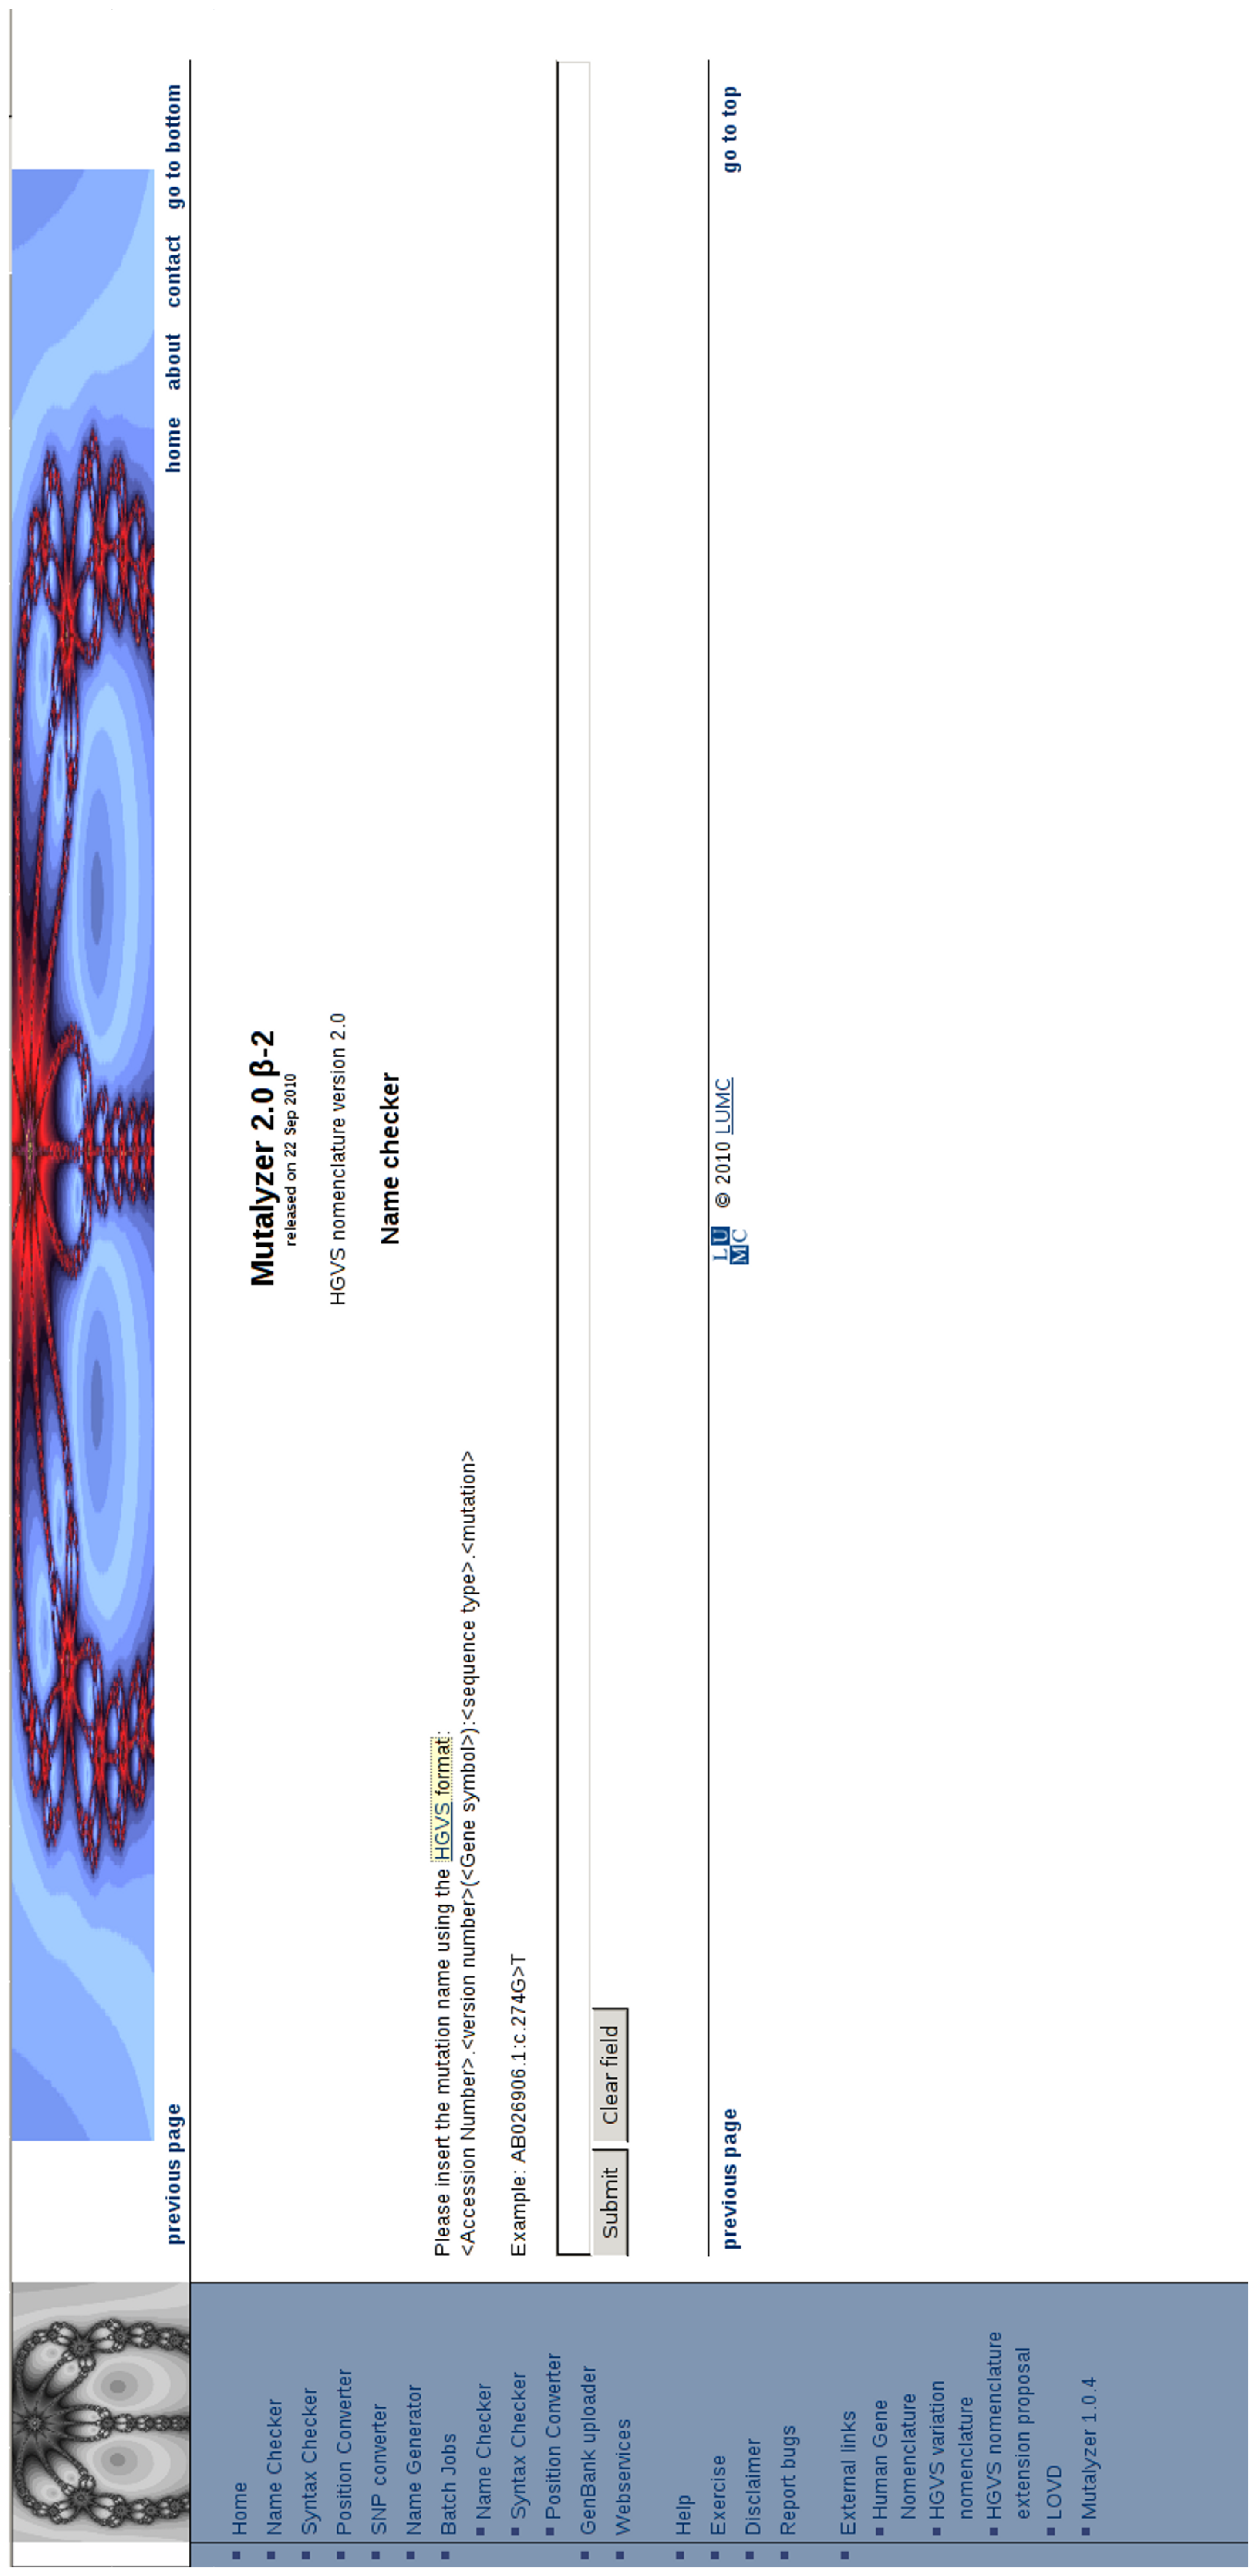
\includegraphics[angle=270, scale=0.26]{shot1}}
\end{slide}
\begin{slide}
\rput(8.5,0){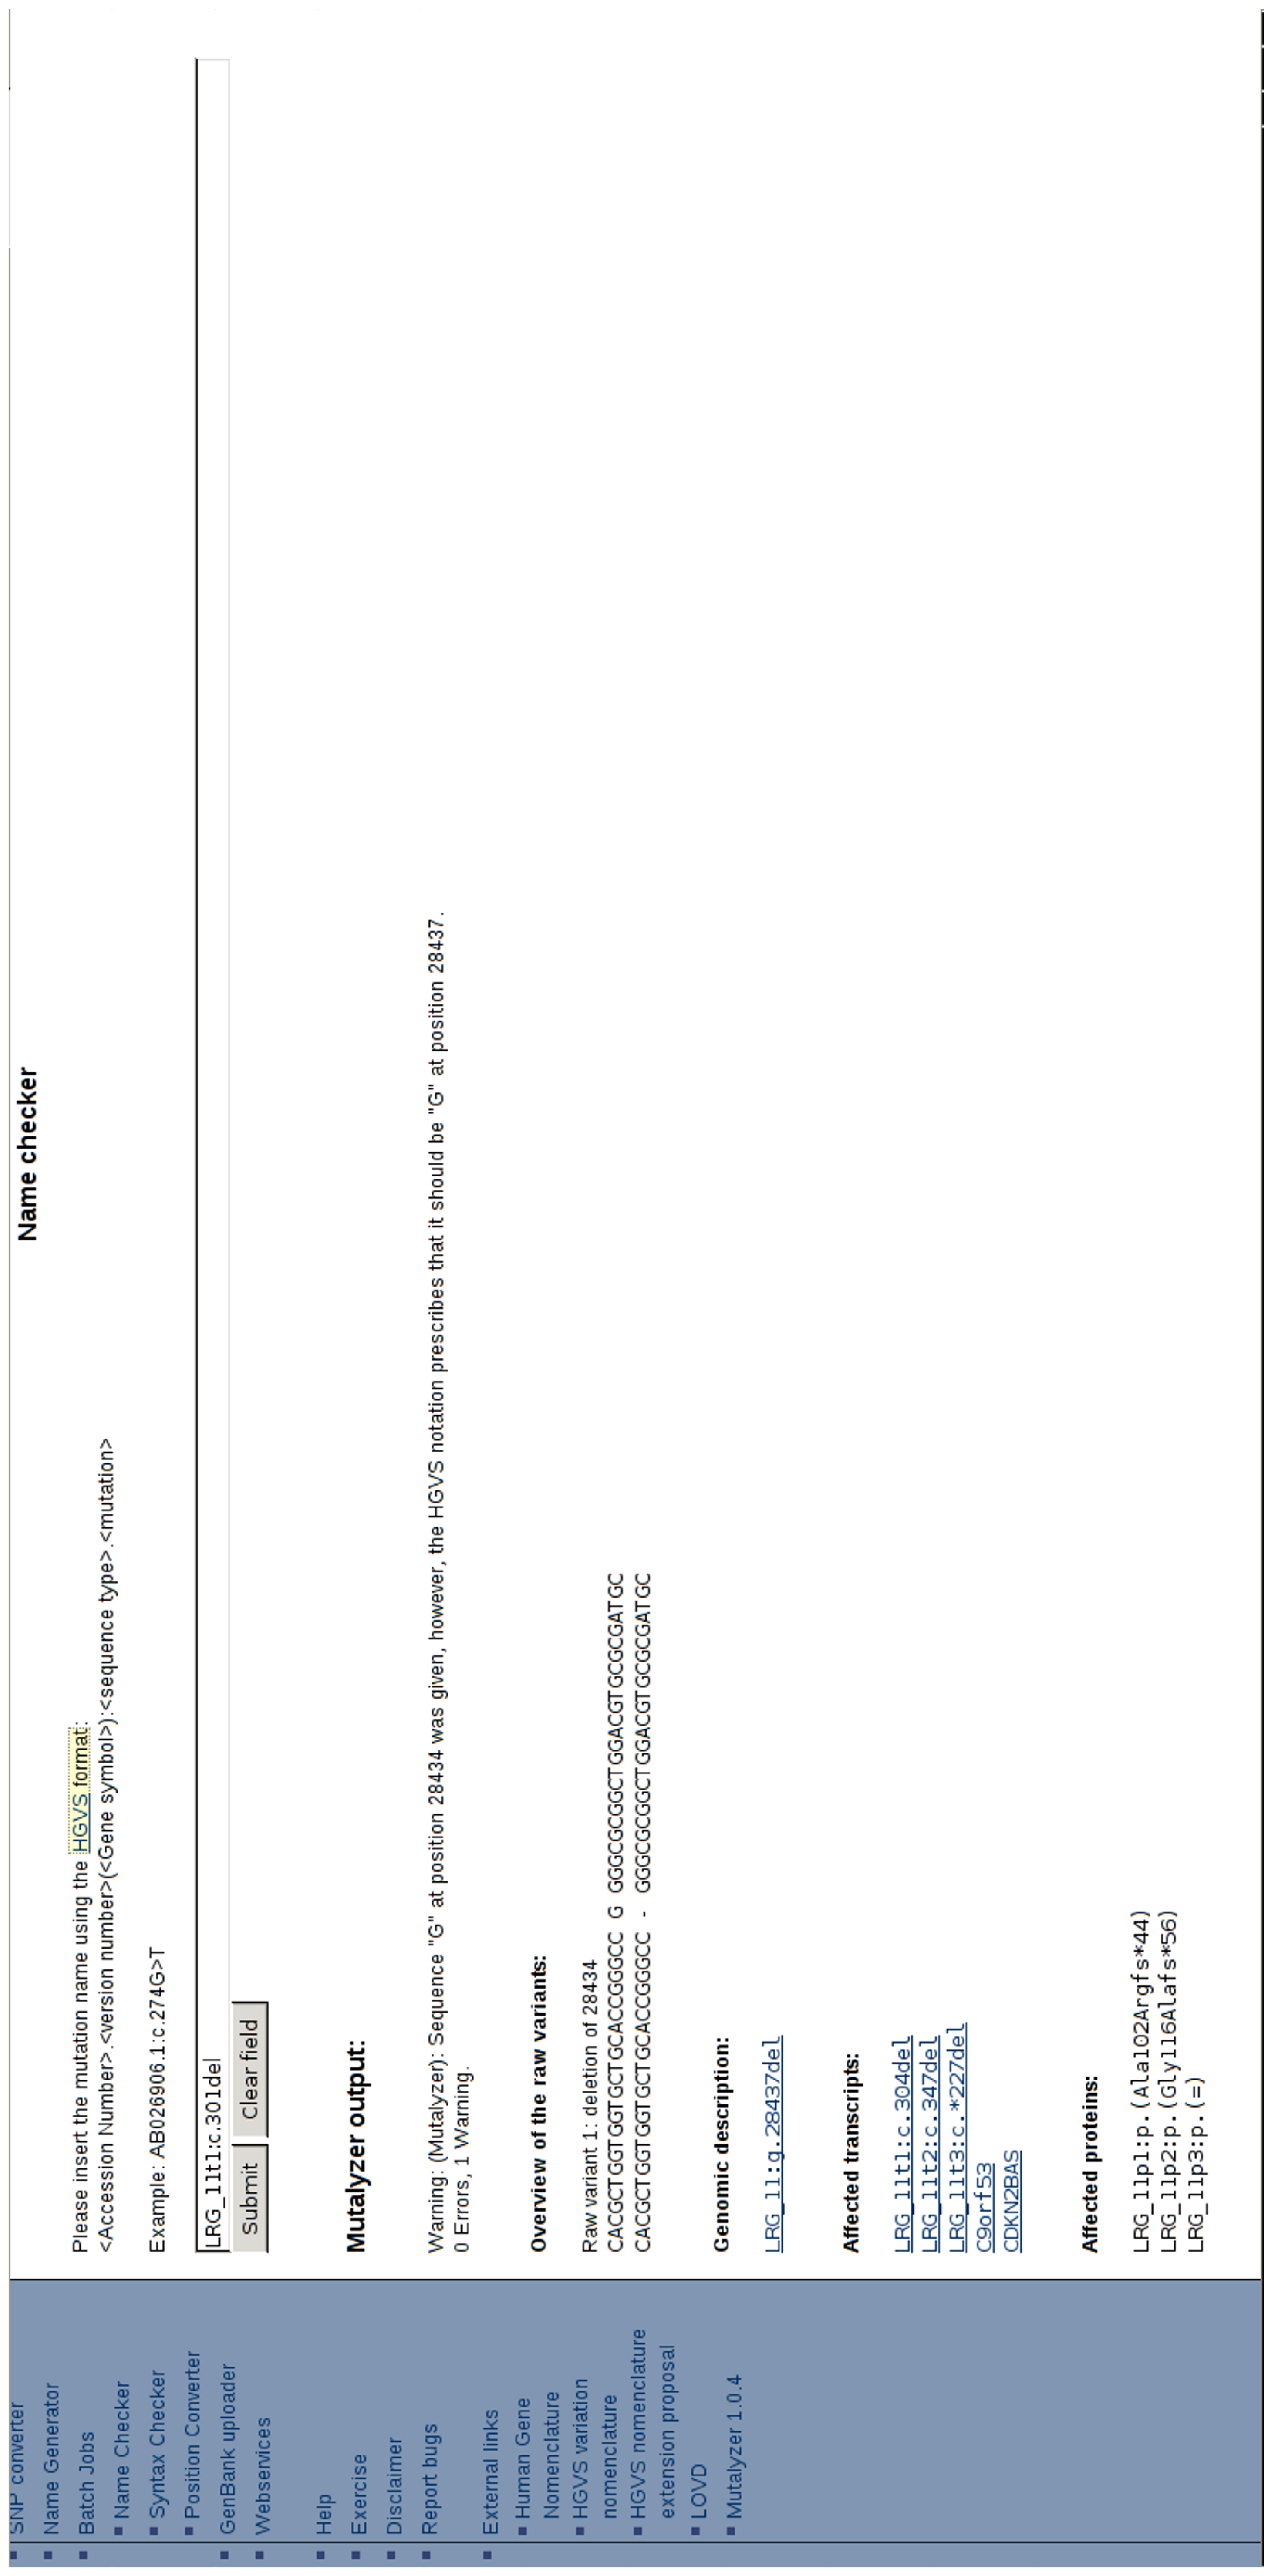
\includegraphics[angle=270, scale=0.26]{shot2}}
\end{slide}
\begin{slide}
\rput(8.5,0){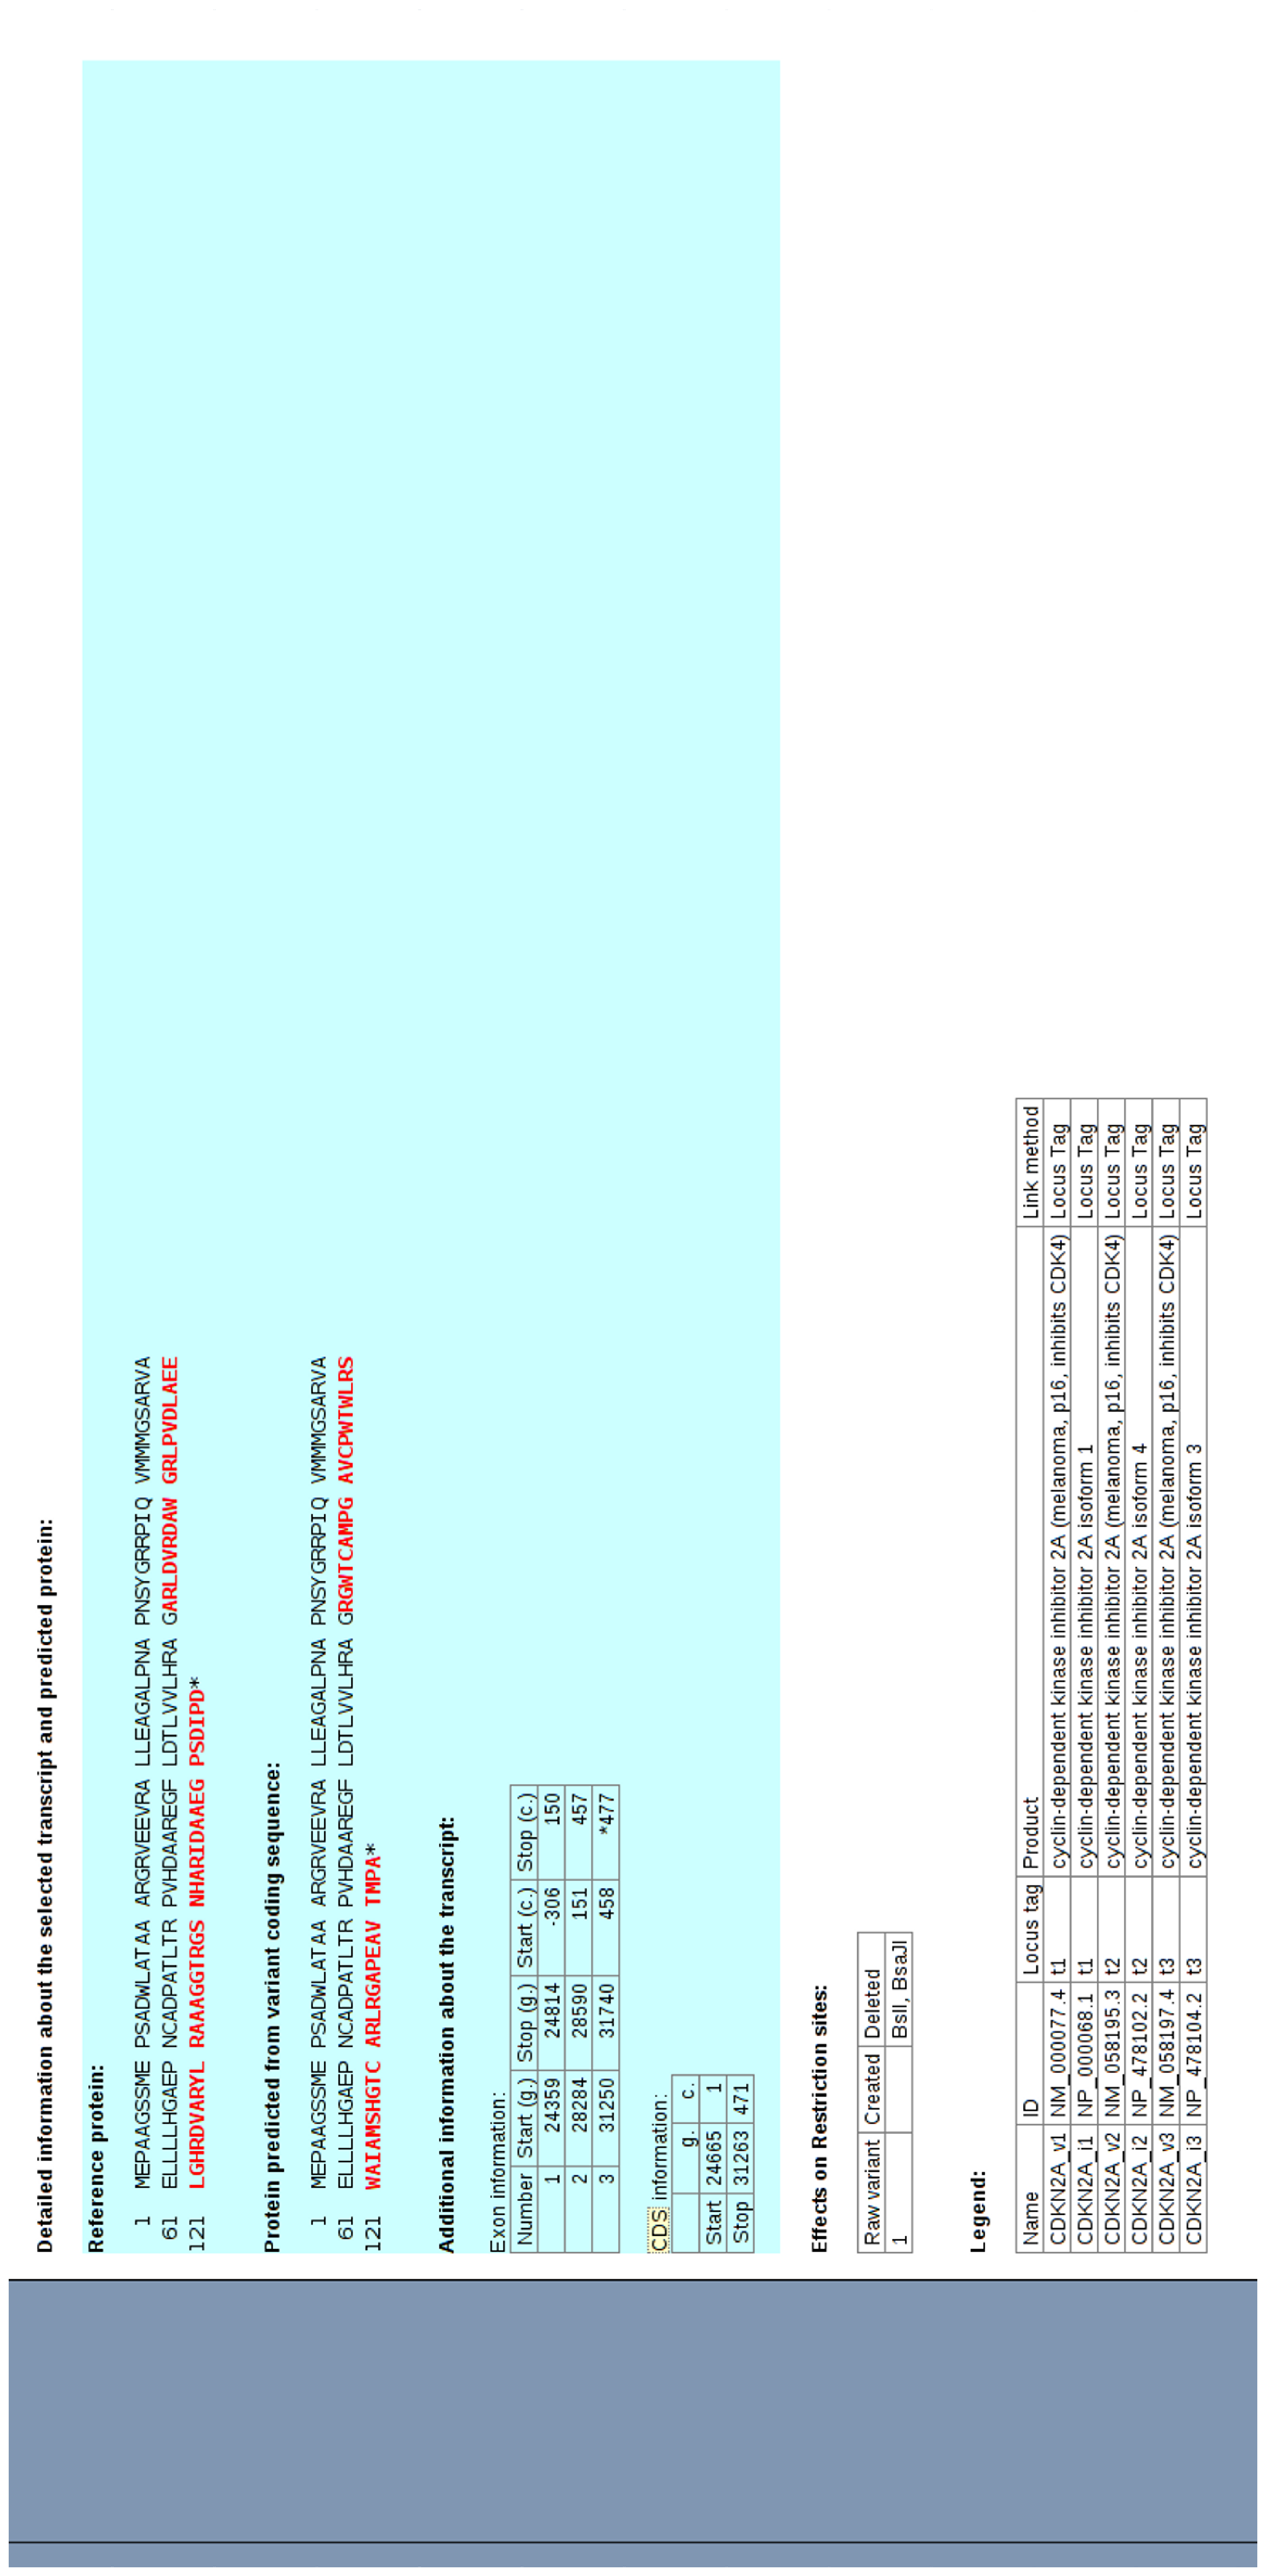
\includegraphics[angle=270, scale=0.26]{shot3}}
\end{slide}
\begin{slide}
\rput(8.5,0){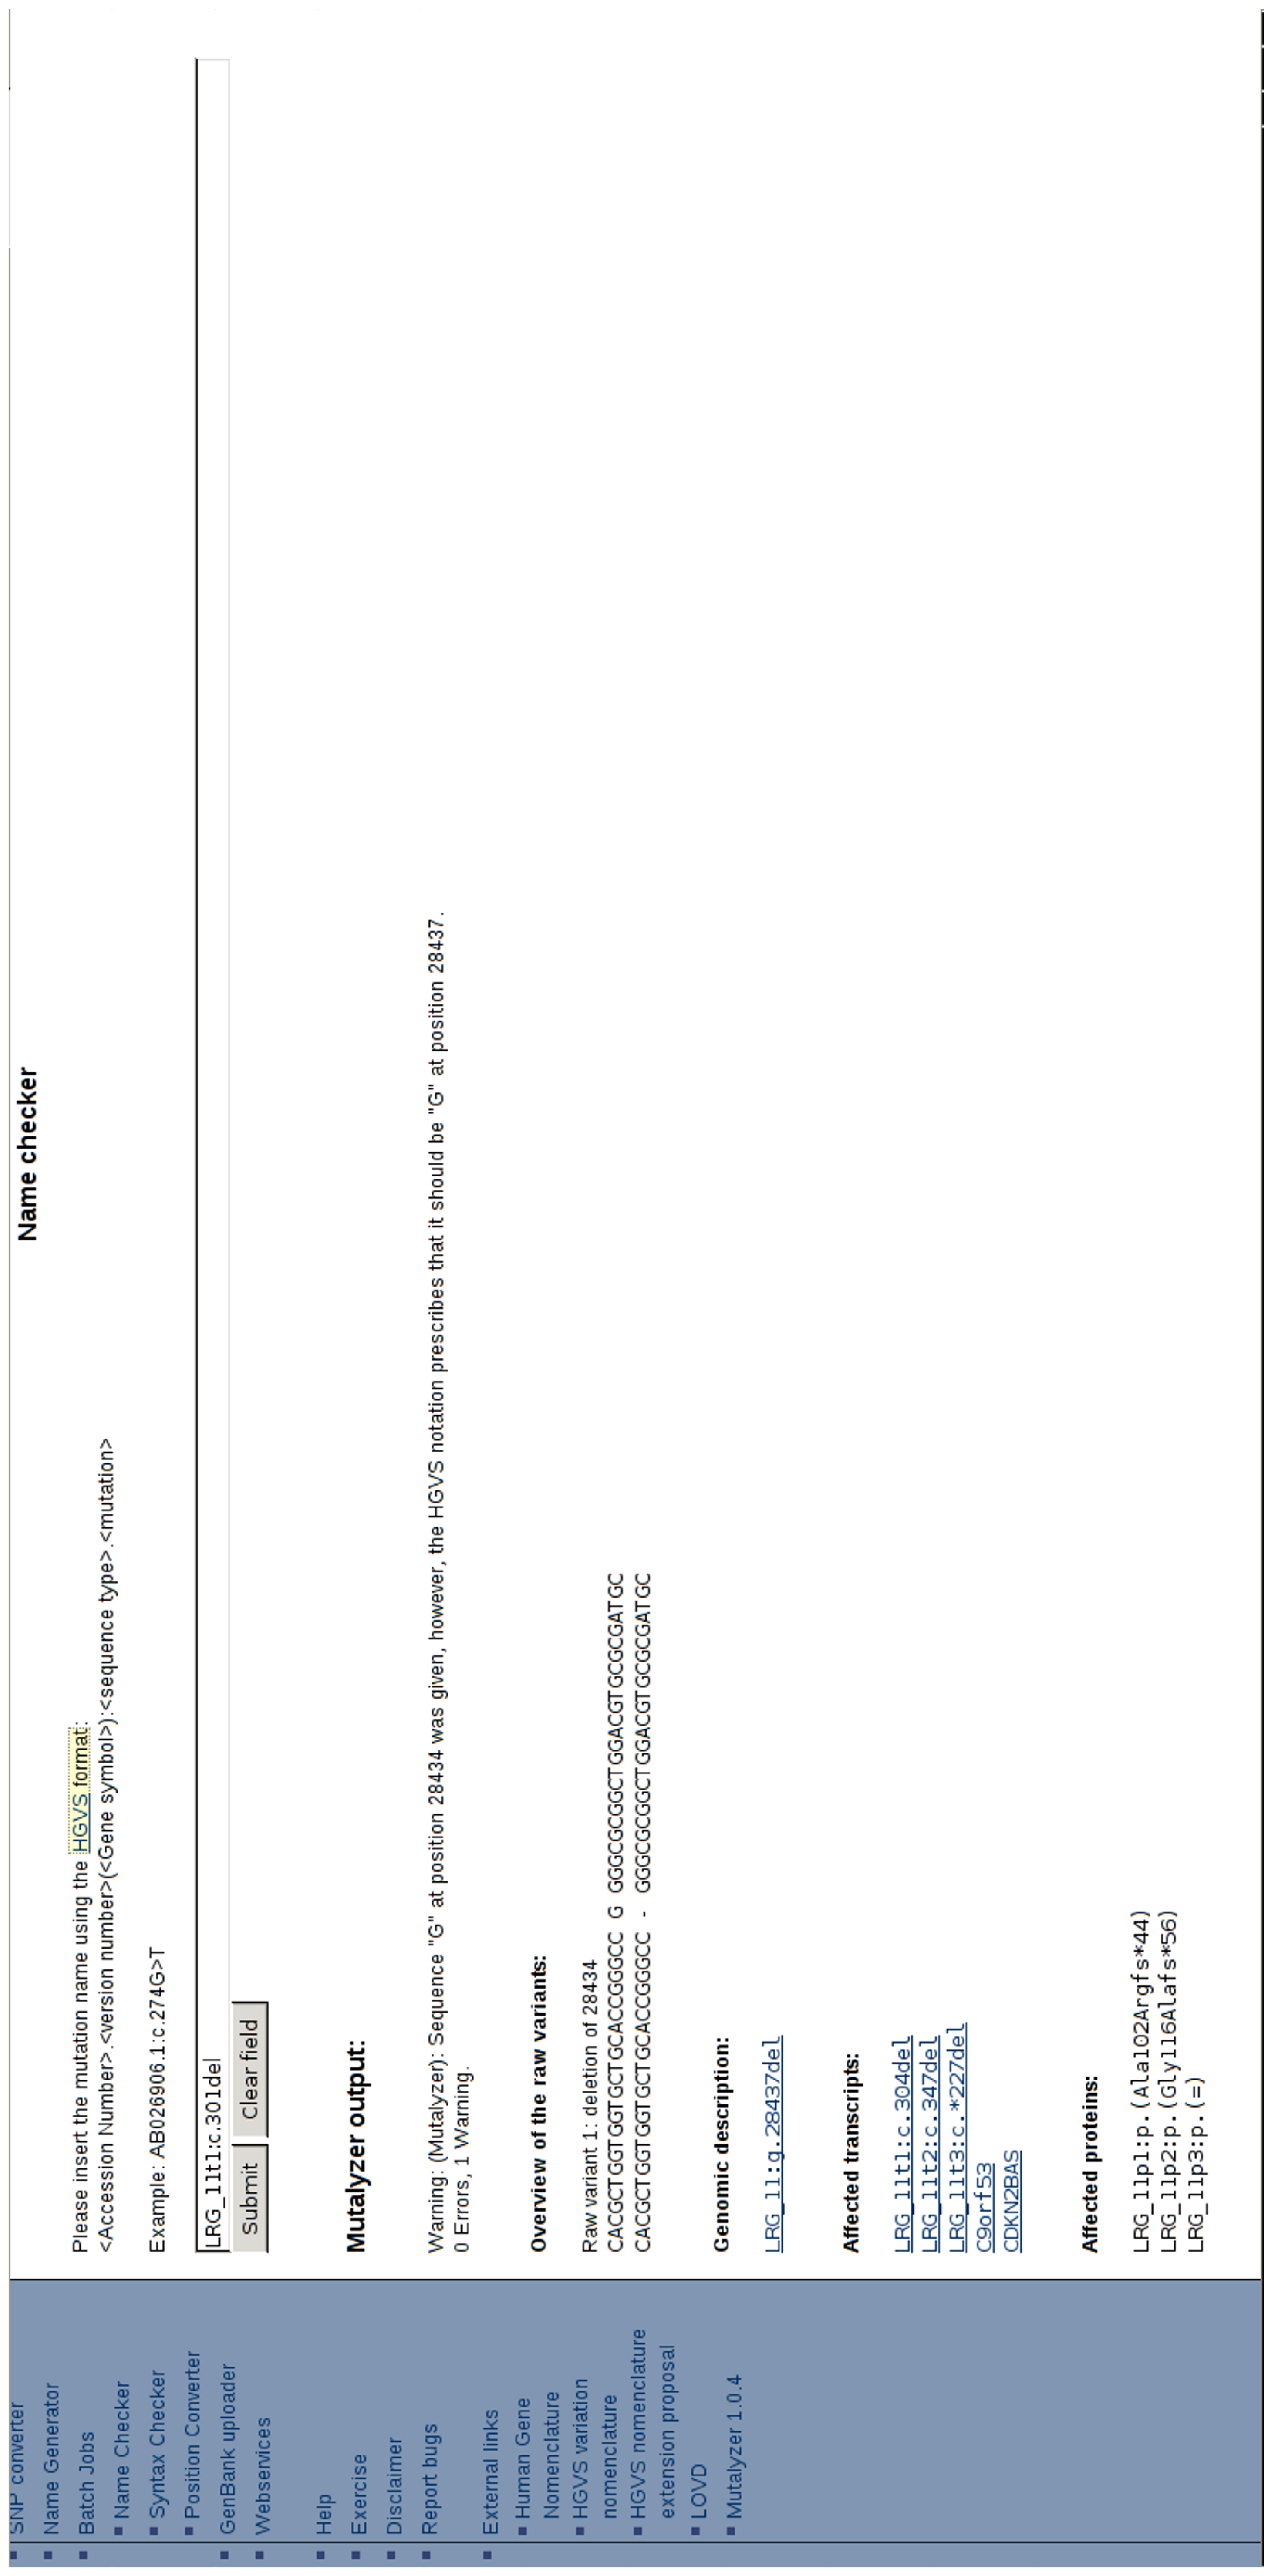
\includegraphics[angle=270, scale=0.26]{shot2}}
\end{slide}
\begin{slide}
\rput(8.5,0){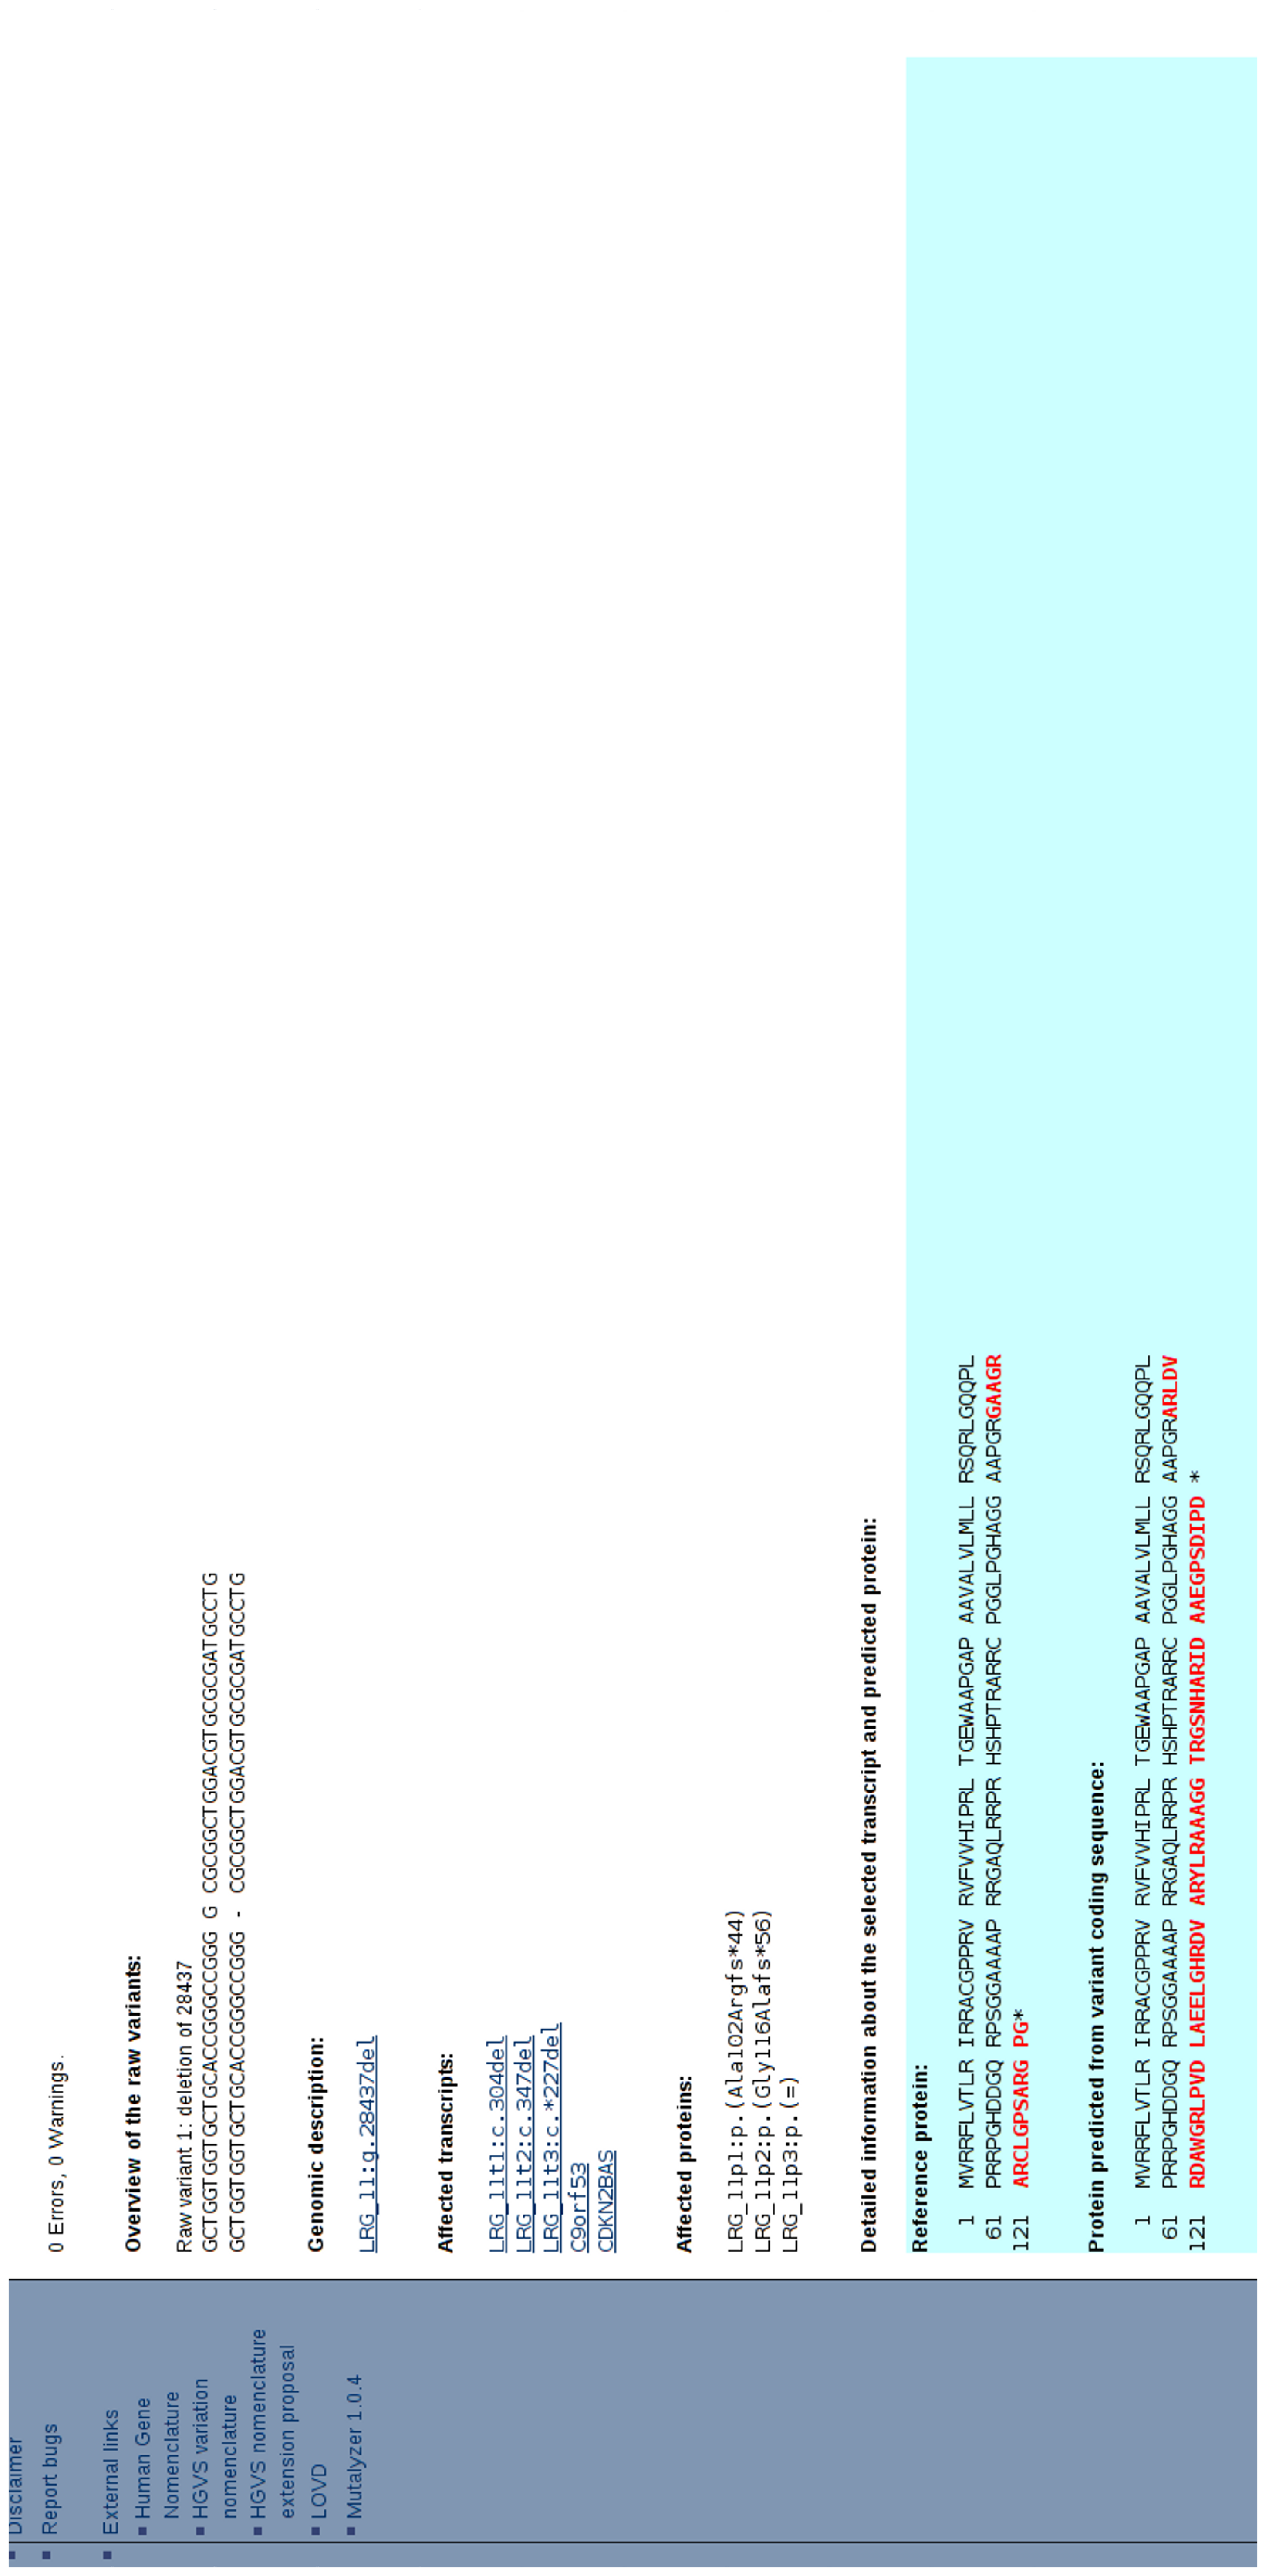
\includegraphics[angle=270, scale=0.26]{shot4}}
\end{slide}

\begin{slide}
\rput(11.4,0.6){\includegraphics[scale=0.1]{Gen2Phen}}
\slideheading{Questions?}
\begin{center}
Acknowledgements

\vspace*{1cm}
Gerben Stouten\\
Peter Taschner\\
Johan den Dunnen\\
Ivo Fokkema\\
Gerard Schaafsma\\
Jacopo Celli\\
\end{center}
\vfill
\label{LastPage}
\end{slide}

\end{document}
